\documentclass{beamer}
\usetheme{Berlin}
\useoutertheme{miniframes}
\usepackage{mathtools}
\usepackage{amssymb}
\usepackage{amsthm}
\usepackage{physics}
\usepackage{stmaryrd}
\usepackage{bbm}
\usepackage{graphicx}
\usepackage{adjustbox}
\usepackage{hyperref}
\usepackage{tikz}
\usepackage{verbatim}
\usetikzlibrary{angles, quotes}
\usetikzlibrary{calc}
\usepackage{pgfplots}
\usepackage{subcaption}
\usepackage{graphicx}
\usepackage{parskip}
\usepackage{mdframed}
\usepackage{biblatex}
\addbibresource{refs.bib}
\title{Représentations textuelles et plongements sémantiques : une application pour l'analyse de sentiment/dissertation}
\author{MARIE Clément, SAMAHA Elio, XIA Tianxiang \newline \newline Encadré par Mr. Olivier Schwander}
\usepackage{setspace}
\linespread{0.7}
\setlength{\itemsep}{4pt}
\setbeamertemplate{itemize/enumerate body begin}{\vspace{0pt}}
\setbeamertemplate{navigation symbols}{}
\setbeamertemplate{footline}{%
  \hspace*{\fill}%
  \usebeamercolor[fg]{page number in head/foot}%
  \usebeamerfont{page number in head/foot}%
  \insertframenumber\,/\,\inserttotalframenumber\kern1em\vskip2pt%
}

\setbeamercolor{section in head/foot}{fg=white}
    \setbeamercolor{section in head/foot shaded}{fg=white}
\usepackage{caption}
\captionsetup[figure]{labelformat=empty}
\captionsetup[table]{labelformat=empty}

\begin{document}
\frame{\titlepage}

\begin{frame}
    \tableofcontents
\end{frame}
\section{Introduction}
\begin{frame}
\frametitle{Introduction - Motivation}

\begin{tikzpicture}[remember picture,overlay]
  % Change the y-coordinate to adjust the vertical position
  \node[anchor=north east,inner sep=0pt] at (current page.north east) {\includegraphics[width=7.25cm]{tric_trac_pic.png}};
\end{tikzpicture}

\vspace{2cm}

\begin{itemize}
  \item Site web Tric Trac: site communautaire autour des jeux de société
  \item Collecte d'avis et de notes des utilisateurs sur les jeux
  \item Traitement de données par représentation vectorielle de mots: analyse multidimensionnelle
  \item Apprentissage statistique (avis en paramètre et la classe comme variable prédite), algorithmes de classification
  \item Enjeux pour l'entreprise   
\end{itemize}
\end{frame}

\begin{frame}
\frametitle{Analyse descriptive des notes: anticipation du problème}

\centering
\includegraphics[width=7cm]{hist_plot_count.png}

\begin{itemize}
  \item Tendance positive des notes: déséquilibre de classes
  \item Solution: harmoniser la répresentation positive/négative
  \item Adapter en conséquence les métriques d'évaluation 
\end{itemize}
\end{frame}

% \section{Représentations et algorithmes}

% \begin{frame}
% \frametitle{Représentation vectorielle des documents}
% \begin{itemize}
%     \item Besoin d'une répresentation numérique: structurée et quantifiable 
%     \item Prétraitement (ponctuation, Stemming, stopwords, etc.)
% \end{itemize}


% \begin{figure}[htbp]
%   \centering
%   \begin{subfigure}{0.4\textwidth}
%     \centering
%     \includegraphics[width=\textwidth]{bag_words.jpeg} % Adjust width and image filename as needed
%     \caption{Bag of words}
%     \label{fig:image1}
%   \end{subfigure}
%   \hfill
%   \begin{subfigure}{0.4\textwidth}
%     \centering
%     \includegraphics[width=\textwidth]{ohe.png} % Adjust width and image filename as needed
%     \caption{One hot encoding}
%     \label{fig:image2}
%   \end{subfigure}
%   \caption{Two Images}
%   \label{fig:two_images}
% \end{figure}

% \end{frame}

\begin{frame}[fragile]
\frametitle{Représentation vectorielle des documents}
\begin{itemize}
    \item Besoin d'une répresentation numérique: structurée et quantifiable 
    \item Prétraitement (ponctuation, stemming, stopwords, etc.)
    \item Plongement lexical (One hot encoding ou bag of words ou tf-idf, etc.)
\end{itemize}
\textbf{Exemple:}
\begin{verbatim}
J'avais peur que les extensions s'éssouflent à terme...
->
['peur', 'extens', 'éssouflent', 'term', ...]
->
[0, 0, 1.2, 1, ...]
\end{verbatim}
\end{frame}

\frame[shrink]{\frametitle{Plongement lexical}
\begin{figure}
\centering
\includegraphics[width=10cm]{puppy.pdf}
\end{figure}
\textbf{Avantages}:
  \begin{itemize}
    \item Préserve la signification sémantique des mots dans le document.
    \item Considère moins les mots non-important. (tf-idf)
  \end{itemize}
\textbf{Inconvénients}:
  \begin{itemize}
    \item Ignore la grammaire et l'ordre des mots, entraînant une perte d'informations contextuelles.
    \item Augmente la dimensionnalité et la parcimonie de la représentation vectorielle.
  \end{itemize}
}

% \frame{\frametitle{Sac de Mots (Bag of Words)}
% \begin{itemize}
%   \item {Exemple}:
%   \begin{itemize}
%     \item Phrase 1: "Le chat dort sur le chat."
%     \item Phrase 2: "Le chien saute."
%   \end{itemize}
% \end{itemize}

% \begin{center}
% \begin{tabular}{|c|c|c|c|c|}
%   \hline
%   & \textbf{chat} & \textbf{chien} & \textbf{dort} & \textbf{saute} \\
%   \hline
%   \textbf{Phrase 1} & 2 & 0 & 1 & 0 \\
%   \hline
%   \textbf{Phrase 2} & 0 & 1 & 0 & 1 \\
%   \hline
% \end{tabular}
% \end{center}

% \begin{itemize}
%   \item \textbf{Avantages}:
%   \begin{itemize}
%     \item Simple et facile à implémenter.
%     \item Préserve la signification sémantique des mots dans le document.
%   \end{itemize}
%   \item \textbf{Inconvénients}:
%   \begin{itemize}
%     \item Ignore la grammaire et l'ordre des mots, entraînant une perte d'informations contextuelles.
%     \item Augmente la dimensionnalité et la parcimonie de la représentation vectorielle.
%   \end{itemize}
% \end{itemize}

% }

\begin{frame}{Distances: Cosinus et Euclidienne}
\begin{minipage}{0.55\textwidth}
\begin{itemize}
\setlength\itemsep{1em} % ajustez la valeur pour augmenter/diminuer l'espacement
\item \textbf{Distance Euclidienne:}
\item[] $D(u, v) := \sqrt{\sum_{i=1}^{n} (u_i - v_i)^2}$
\item \textbf{Distance Cosinus:}
\item[] $D(u, v) :=1-S(u, v)$
\item[] Où $S(u, v) := \cos(\theta)=\frac{u \cdot v}{|u||v|}$
\item[] C'est la similarité cosinus entre $u$ et $v$
\end{itemize}
\end{minipage}
\hfill
\begin{minipage}{0.4\textwidth}
\begin{figure}
\centering
\tikzset{every picture/.style={line width=0.75pt}} %set default line width to 0.75pt        

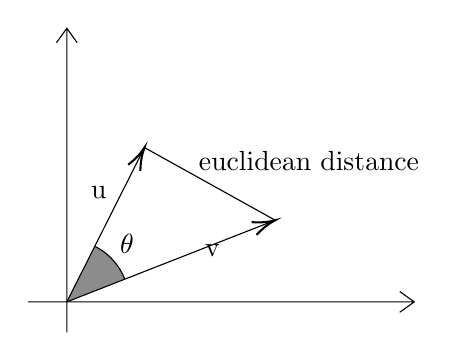
\begin{tikzpicture}[x=0.75pt,y=0.75pt,yscale=-1,xscale=1]
%uncomment if require: \path (0,300); %set diagram left start at 0, and has height of 300

%Shape: Axis 2D [id:dp9247573707891508] 
\draw  (50,199.85) -- (236,199.85)(68.6,68) -- (68.6,214.5) (229,194.85) -- (236,199.85) -- (229,204.85) (63.6,75) -- (68.6,68) -- (73.6,75)  ;
%Straight Lines [id:da4418715205409134] 
\draw    (68.6,199.85) -- (167.14,161.23) ;
\draw [shift={(169,160.5)}, rotate = 158.6] [color={rgb, 255:red, 0; green, 0; blue, 0 }  ][line width=0.75]    (10.93,-3.29) .. controls (6.95,-1.4) and (3.31,-0.3) .. (0,0) .. controls (3.31,0.3) and (6.95,1.4) .. (10.93,3.29)   ;
%Straight Lines [id:da9719047623164807] 
\draw    (68.6,199.85) -- (95.55,146.27) -- (105.1,127.29) ;
\draw [shift={(106,125.5)}, rotate = 116.7] [color={rgb, 255:red, 0; green, 0; blue, 0 }  ][line width=0.75]    (10.93,-3.29) .. controls (6.95,-1.4) and (3.31,-0.3) .. (0,0) .. controls (3.31,0.3) and (6.95,1.4) .. (10.93,3.29)   ;
%Shape: Arc [id:dp7509394088510173] 
\draw  [draw opacity=0][fill={rgb, 255:red, 0; green, 0; blue, 0 }  ,fill opacity=0.45 ] (82.33,173.17) .. controls (87.77,175.97) and (92.42,180.45) .. (95.38,186.34) .. controls (95.78,187.12) and (96.14,187.92) .. (96.46,188.72) -- (68.6,199.85) -- cycle ; \draw   (82.33,173.17) .. controls (87.77,175.97) and (92.42,180.45) .. (95.38,186.34) .. controls (95.78,187.12) and (96.14,187.92) .. (96.46,188.72) ;  
%Straight Lines [id:da2404981848512595] 
\draw    (106,125.5) -- (169,160.5) ;

% Text Node
\draw (93,166) node [anchor=north west][inner sep=0.75pt]   [align=left] {$\displaystyle \theta $};
% Text Node
\draw (131,126) node [anchor=north west][inner sep=0.75pt]   [align=left] {euclidean distance};
% Text Node
\draw (79,143) node [anchor=north west][inner sep=0.75pt]   [align=left] {u};
% Text Node
\draw (134,171) node [anchor=north west][inner sep=0.75pt]   [align=left] {v};


\end{tikzpicture}
\caption{Illustration de Distance Cosinus et Euclidienne}
\end{figure}
\end{minipage}
\end{frame}

\section{K-Plus Proches Voisins}

\begin{frame}{K-Plus Proches Voisins (KPP ou KNN)}
  \begin{columns}
    \begin{column}{0.5\textwidth}
      \textbf{Avantages :}
      \begin{itemize}
        \setlength\itemsep{0.5em}
        \item Simple et facile à implémenter.
        \item Méthode non paramétrique.
        \item Convient à la fois pour les tâches de classification et de régression.
      \end{itemize}
      \vspace{1em}
      \textbf{Inconvénients :}
      \begin{itemize}
        \setlength\itemsep{0.5em}
        \item Coûteux en calcul pour les grands ensembles de données.
        \item Sensible au choix de k et de la métrique de distance.
        \item Performances médiocres avec des données de grande dimension.
      \end{itemize}
    \end{column}
    \begin{column}{0.6\textwidth}
      \begin{center}
        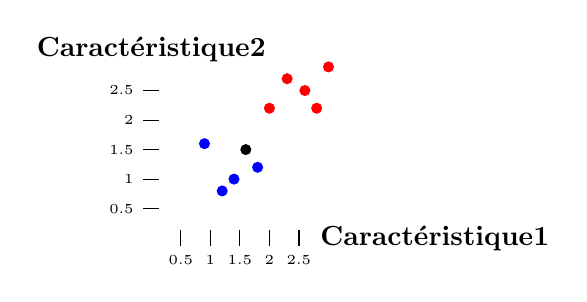
\begin{tikzpicture}[scale=1]
          % Points bleus
          \foreach \point in {(0.9,0.6), (1.35,0.9), (0.675,1.2), (1.05,0.75)} {
            \fill[blue] \point circle (2pt);
          }
          
          % Points rouges
          \foreach \point in {(1.5,1.65), (1.95,1.875), (1.725,2.025), (2.25,2.175), (2.1,1.65)} {
            \fill[red] \point circle (2pt);
          }

          % Point noir (sujet test)
          \fill[black] (1.2,1.125) circle (2pt);
          
          % Étiquettes des axes
          \node at (3.6,0) {{\textbf{Caractéristique1}}};
          \node at (0,2.4) {{\textbf{Caractéristique2}}};
          
          % Graduations des axes
          \draw (0.375,0.1) -- (0.375,-0.1) node[below] {\tiny{0.5}};
          \draw (0.75,0.1) -- (0.75,-0.1) node[below] {\tiny{1}};
          \draw (1.125,0.1) -- (1.125,-0.1) node[below] {\tiny{1.5}};
          \draw (1.5,0.1) -- (1.5,-0.1) node[below] {\tiny{2}};
          \draw (1.875,0.1) -- (1.875,-0.1) node[below] {\tiny{2.5}};
          
          \draw (0.1,0.375) -- (-0.1,0.375) node[left] {\tiny{0.5}};
          \draw (0.1,0.75) -- (-0.1,0.75) node[left] {\tiny{1}};
          \draw (0.1,1.125) -- (-0.1,1.125) node[left] {\tiny{1.5}};
          \draw (0.1,1.5) -- (-0.1,1.5) node[left] {\tiny{2}};
          \draw (0.1,1.875) -- (-0.1,1.875) node[left] {\tiny{2.5}};
        \end{tikzpicture}
      \end{center}
    \end{column}
  \end{columns}
\end{frame}



\begin{frame}
\frametitle{KNN Analysis (1)}

\begin{figure}[h]
  \centering
  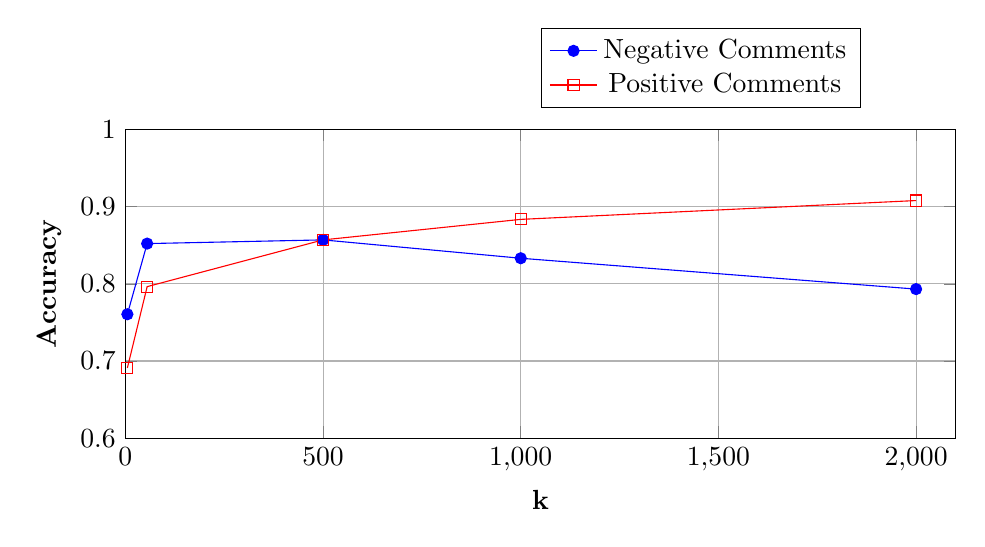
\begin{tikzpicture}
      \begin{axis}[
          xlabel={\textbf{k}},
          ylabel={\textbf{Accuracy}},
          xmin=0, xmax=2100,
          ymin=0.6, ymax=1,
          xtick={0,500,1000,1500,2000},
          ytick={0.6,0.7,0.8,0.9,1},
          legend style={at={(0.5,1.2)}, anchor=west}, % Adjust this line
          grid=both,
          grid style={line width=0.2pt, draw=gray!30},
          major grid style={line width=0.4pt,draw=gray!60},
          height=5.5cm,
          width=1\textwidth
      ]
      \addplot[color=blue, mark=*] coordinates {
          (5,0.7606)
          (55,0.8522)
          (500,0.857)
          (1000,0.8332)
          (2000,0.7932)
      };
      \addplot[color=red, mark=square] coordinates {
          (5,0.691)
          (55,0.7964)
          (500,0.857)
          (1000,0.8836)
          (2000,0.908)
      };
      \legend{Negative Comments, Positive Comments}
      \end{axis}
  \end{tikzpicture}
  \caption{k nearest neighbor on balanced data (5000 positive/negative comments)}
  \label{fig:KNN1}
\end{figure}
\end{frame}

\begin{frame}[shrink]{KNN Analysis (2)}
\begin{figure}
    \begin{minipage}{0.49\textwidth}
    \centering
    \includegraphics[width=\linewidth]{balancek50.png}
    \subcaption{$k=50$}
    \end{minipage}
    \centering
    \begin{minipage}{0.49\textwidth}
    \includegraphics[width=\linewidth]{balancek500.png}
    \subcaption{$k=500$}
    \end{minipage}
\end{figure}

\begin{table}
  \centering
  \begin{tabular}{@{}ccccc@{}}
  \hline
  Class & Precision & Recall & F1-Score & Support \\
  \hline
  False (negative comments) & 0.23 & 0.91 & 0.37 & 1789 \\
  True (positive comments) & 0.99 & 0.76 & 0.86 & 22520 \\
  \hline
  \multicolumn{5}{c}{Accuracy = 0.77} \\
  \hline
  \end{tabular}
  \caption{Classification report with undersampling (balance = 1, k = 500)}
  \label{tab:KNN}
\end{table}
\end{frame}

\begin{frame}[shrink]
\frametitle{KNN Analysis with Different Options}

\begin{figure}[h]
  \centering
  \begin{tabular}{|c|c|c|c|}
  \hline
  & \textbf{BoW} & \textbf{tf-idf} & \textbf{One-hot} \\ \hline
  \textbf{Euclidean} & 0.7642 (1) & 0.7425 (113) & 0.6864 (5) \\ \hline
  \textbf{Cosine} &  0.7725 (1) & 0.7771 (1) & 0.6864 (5) \\ \hline
  \end{tabular}
  \caption{Comparative Accuracy Results, (k)}
  \label{tab:accuracy}
\end{figure}

\begin{figure}[h]
  \centering
  \includegraphics[width=6cm]{accuracy_plot.png}
  \caption{Variation of accuracy with k (KNN, euclidean distance, BoW)}
  \label{fig:KNNOptions}
\end{figure}
\end{frame}

\section{Naive Bayes}

\begin{frame}
\frametitle{Naive Bayes}
\begin{itemize}
    \item Bag of words: décompte des occurrences de mots dans le corpus (rép. vectorielle pas nécéssaire)
    \item Algorithme de classification probabiliste
    \item Naif car suppose que les variables sont indépendantes
    \item Probabilités conditionnelles par classe
    \item Classification où la classe prédite maximise la probabilité
\end{itemize}

\begin{figure}
    \begin{minipage}[b]{0.60\textwidth}
        \centering
        \includegraphics[width=\textwidth]{nb.png} 
    \end{minipage}
\end{figure}

\end{frame}

\begin{frame}{Naive Bayes - Metrics}
\begin{figure}[H]
    \begin{minipage}[c]{0.45\textwidth}
        \centering
        \includegraphics[width=1.2\textwidth]{nb_mat_no_undersampling.png} 
        \subcaption{Pas d'undersampling}
    \end{minipage}\hfill
    \begin{minipage}[c]{0.45\textwidth}
        \centering
        \includegraphics[width=1.2\textwidth]{nb_mat_undersampling.png}
        \subcaption{Undersampling}
    \end{minipage}
    \caption{Matrices de confusion et métriques associées}
\end{figure}

\begin{table}
\centering
\resizebox{0.6\textwidth}{!}{
\begin{tabular}{cccc}
  & F1 Pos. & F1 Neg. & Accuracy \\
  \hline
  Undersampling & 0.83 & 0.50 & 0.74 \\
  No undersampling & 0.93 & 0.40 & 0.88 \\
\end{tabular}
}
\label{subfig:scores}
\end{table}
\end{frame}


\section{Homologie persistente}

\begin{frame}{Motivation - Représentation par homologie persistente}

Maintenant on veut une méthode qui

\begin{itemize}
    \item considère la structure des phrases
dans un document (qui a été ignorée);
    \item n'a pas de paramètre qui dépend des données d'entrainement. (plus robust)
\end{itemize}

Pour la prédiction du sentiment, cela n'a pas beaucoup d'avantage par rapport à KNN ou Naive Bayes. On change à une tâche plus appropriée : analyser la richesse des structures dans une dissertation.

\end{frame}

\begin{frame}[fragile, shrink]{Introduction}
\begin{figure}[H]
  \begin{minipage}{0.49\textwidth}
  \scalebox{0.45}{\tikzset{every picture/.style={line width=0.75pt}} %set default line width to 0.75pt        

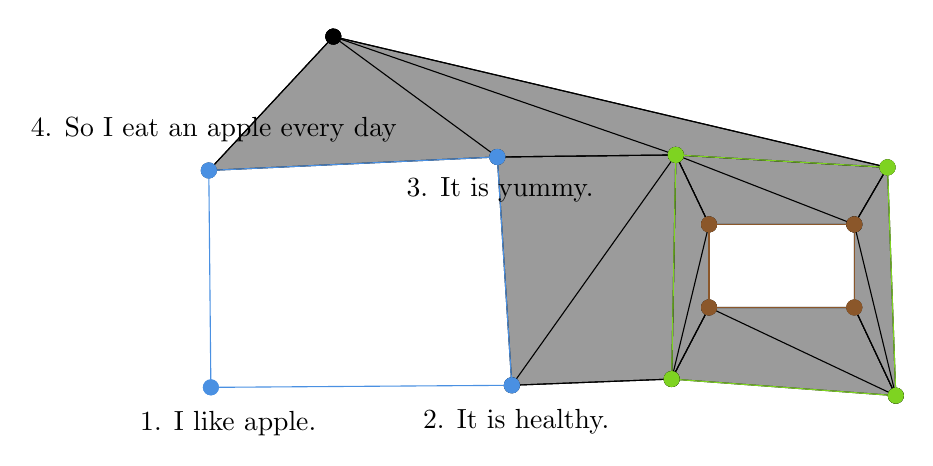
\begin{tikzpicture}[x=0.75pt,y=0.75pt,yscale=-1,xscale=1]
%uncomment if require: \path (0,300); %set diagram left start at 0, and has height of 300

%Shape: Polygon [id:ds506045927728886] 
\draw  [fill={rgb, 255:red, 155; green, 155; blue, 155 }  ,fill opacity=1 ] (337,211.5) -- (355,177) -- (425,177) -- (445,219.5) -- cycle ;
%Shape: Polygon [id:ds373063136182463] 
\draw  [fill={rgb, 255:red, 155; green, 155; blue, 155 }  ,fill opacity=1 ] (441,109.5) -- (425,137) -- (355,137) -- (339,103.5) -- cycle ;
%Shape: Polygon [id:ds04357467087348055] 
\draw  [fill={rgb, 255:red, 155; green, 155; blue, 155 }  ,fill opacity=1 ] (445,219.5) -- (425,177) -- (425,137) -- (441,109.5) -- cycle ;
%Shape: Polygon [id:ds8597694080078087] 
\draw  [fill={rgb, 255:red, 155; green, 155; blue, 155 }  ,fill opacity=1 ] (339,103.5) -- (355,137) -- (355,177) -- (337,211.5) -- cycle ;

%Straight Lines [id:da7958699538877538] 
\draw    (339,103.5) -- (425,137) ;
\draw [shift={(425,137)}, rotate = 21.28] [color={rgb, 255:red, 0; green, 0; blue, 0 }  ][fill={rgb, 255:red, 0; green, 0; blue, 0 }  ][line width=0.75]      (0, 0) circle [x radius= 3.35, y radius= 3.35]   ;
\draw [shift={(339,103.5)}, rotate = 21.28] [color={rgb, 255:red, 0; green, 0; blue, 0 }  ][fill={rgb, 255:red, 0; green, 0; blue, 0 }  ][line width=0.75]      (0, 0) circle [x radius= 3.35, y radius= 3.35]   ;
%Straight Lines [id:da37382810612047734] 
\draw    (425,137) -- (445,219.5) ;
\draw [shift={(445,219.5)}, rotate = 76.37] [color={rgb, 255:red, 0; green, 0; blue, 0 }  ][fill={rgb, 255:red, 0; green, 0; blue, 0 }  ][line width=0.75]      (0, 0) circle [x radius= 3.35, y radius= 3.35]   ;
\draw [shift={(425,137)}, rotate = 76.37] [color={rgb, 255:red, 0; green, 0; blue, 0 }  ][fill={rgb, 255:red, 0; green, 0; blue, 0 }  ][line width=0.75]      (0, 0) circle [x radius= 3.35, y radius= 3.35]   ;
%Straight Lines [id:da33578118329024775] 
\draw    (355,177) -- (445,219.5) ;
\draw [shift={(445,219.5)}, rotate = 25.28] [color={rgb, 255:red, 0; green, 0; blue, 0 }  ][fill={rgb, 255:red, 0; green, 0; blue, 0 }  ][line width=0.75]      (0, 0) circle [x radius= 3.35, y radius= 3.35]   ;
\draw [shift={(355,177)}, rotate = 25.28] [color={rgb, 255:red, 0; green, 0; blue, 0 }  ][fill={rgb, 255:red, 0; green, 0; blue, 0 }  ][line width=0.75]      (0, 0) circle [x radius= 3.35, y radius= 3.35]   ;
%Straight Lines [id:da27555178758587107] 
\draw    (355,137) -- (337,211.5) ;
\draw [shift={(337,211.5)}, rotate = 103.58] [color={rgb, 255:red, 0; green, 0; blue, 0 }  ][fill={rgb, 255:red, 0; green, 0; blue, 0 }  ][line width=0.75]      (0, 0) circle [x radius= 3.35, y radius= 3.35]   ;
\draw [shift={(355,137)}, rotate = 103.58] [color={rgb, 255:red, 0; green, 0; blue, 0 }  ][fill={rgb, 255:red, 0; green, 0; blue, 0 }  ][line width=0.75]      (0, 0) circle [x radius= 3.35, y radius= 3.35]   ;
%Shape: Polygon [id:ds20124875657376728] 
\draw  [fill={rgb, 255:red, 155; green, 155; blue, 155 }  ,fill opacity=1 ] (253,104.5) -- (260,214.5) -- (337,211.5) -- (339,103.5) -- cycle ;
%Shape: Polygon [id:ds3619467537546437] 
\draw  [fill={rgb, 255:red, 155; green, 155; blue, 155 }  ,fill opacity=1 ] (174,46.5) -- (441,109.5) -- (339,103.5) -- (253,104.5) -- (114,111) -- cycle ;
%Straight Lines [id:da5963075508320128] 
\draw    (339,103.5) -- (253,104.5) ;
\draw [shift={(253,104.5)}, rotate = 179.33] [color={rgb, 255:red, 0; green, 0; blue, 0 }  ][fill={rgb, 255:red, 0; green, 0; blue, 0 }  ][line width=0.75]      (0, 0) circle [x radius= 3.35, y radius= 3.35]   ;
\draw [shift={(339,103.5)}, rotate = 179.33] [color={rgb, 255:red, 0; green, 0; blue, 0 }  ][fill={rgb, 255:red, 0; green, 0; blue, 0 }  ][line width=0.75]      (0, 0) circle [x radius= 3.35, y radius= 3.35]   ;
%Straight Lines [id:da8612090103920278] 
\draw    (260,214.5) -- (339,103.5) ;
\draw [shift={(339,103.5)}, rotate = 305.44] [color={rgb, 255:red, 0; green, 0; blue, 0 }  ][fill={rgb, 255:red, 0; green, 0; blue, 0 }  ][line width=0.75]      (0, 0) circle [x radius= 3.35, y radius= 3.35]   ;
\draw [shift={(260,214.5)}, rotate = 305.44] [color={rgb, 255:red, 0; green, 0; blue, 0 }  ][fill={rgb, 255:red, 0; green, 0; blue, 0 }  ][line width=0.75]      (0, 0) circle [x radius= 3.35, y radius= 3.35]   ;
%Straight Lines [id:da9692653745827828] 
\draw    (260,214.5) -- (337,211.5) ;
\draw [shift={(337,211.5)}, rotate = 357.77] [color={rgb, 255:red, 0; green, 0; blue, 0 }  ][fill={rgb, 255:red, 0; green, 0; blue, 0 }  ][line width=0.75]      (0, 0) circle [x radius= 3.35, y radius= 3.35]   ;
\draw [shift={(260,214.5)}, rotate = 357.77] [color={rgb, 255:red, 0; green, 0; blue, 0 }  ][fill={rgb, 255:red, 0; green, 0; blue, 0 }  ][line width=0.75]      (0, 0) circle [x radius= 3.35, y radius= 3.35]   ;
%Straight Lines [id:da7164877740446134] 
\draw    (114,111) -- (174,46.5) ;
\draw [shift={(174,46.5)}, rotate = 312.93] [color={rgb, 255:red, 0; green, 0; blue, 0 }  ][fill={rgb, 255:red, 0; green, 0; blue, 0 }  ][line width=0.75]      (0, 0) circle [x radius= 3.35, y radius= 3.35]   ;
\draw [shift={(114,111)}, rotate = 312.93] [color={rgb, 255:red, 0; green, 0; blue, 0 }  ][fill={rgb, 255:red, 0; green, 0; blue, 0 }  ][line width=0.75]      (0, 0) circle [x radius= 3.35, y radius= 3.35]   ;
%Straight Lines [id:da2125405974487078] 
\draw    (174,46.5) -- (253,104.5) ;
\draw [shift={(253,104.5)}, rotate = 36.29] [color={rgb, 255:red, 0; green, 0; blue, 0 }  ][fill={rgb, 255:red, 0; green, 0; blue, 0 }  ][line width=0.75]      (0, 0) circle [x radius= 3.35, y radius= 3.35]   ;
\draw [shift={(174,46.5)}, rotate = 36.29] [color={rgb, 255:red, 0; green, 0; blue, 0 }  ][fill={rgb, 255:red, 0; green, 0; blue, 0 }  ][line width=0.75]      (0, 0) circle [x radius= 3.35, y radius= 3.35]   ;
%Straight Lines [id:da8884288301278187] 
\draw    (174,46.5) -- (441,109.5) ;
\draw [shift={(441,109.5)}, rotate = 13.28] [color={rgb, 255:red, 0; green, 0; blue, 0 }  ][fill={rgb, 255:red, 0; green, 0; blue, 0 }  ][line width=0.75]      (0, 0) circle [x radius= 3.35, y radius= 3.35]   ;
\draw [shift={(174,46.5)}, rotate = 13.28] [color={rgb, 255:red, 0; green, 0; blue, 0 }  ][fill={rgb, 255:red, 0; green, 0; blue, 0 }  ][line width=0.75]      (0, 0) circle [x radius= 3.35, y radius= 3.35]   ;
%Straight Lines [id:da3878057357434834] 
\draw    (174,46.5) -- (339,103.5) ;
\draw [shift={(339,103.5)}, rotate = 19.06] [color={rgb, 255:red, 0; green, 0; blue, 0 }  ][fill={rgb, 255:red, 0; green, 0; blue, 0 }  ][line width=0.75]      (0, 0) circle [x radius= 3.35, y radius= 3.35]   ;
\draw [shift={(174,46.5)}, rotate = 19.06] [color={rgb, 255:red, 0; green, 0; blue, 0 }  ][fill={rgb, 255:red, 0; green, 0; blue, 0 }  ][line width=0.75]      (0, 0) circle [x radius= 3.35, y radius= 3.35]   ;
%Straight Lines [id:da3895078416872] 
\draw [color={rgb, 255:red, 126; green, 211; blue, 33 }  ,draw opacity=1 ]   (445,219.5) -- (337,211.5) ;
\draw [shift={(337,211.5)}, rotate = 184.24] [color={rgb, 255:red, 126; green, 211; blue, 33 }  ,draw opacity=1 ][fill={rgb, 255:red, 126; green, 211; blue, 33 }  ,fill opacity=1 ][line width=0.75]      (0, 0) circle [x radius= 3.35, y radius= 3.35]   ;
\draw [shift={(445,219.5)}, rotate = 184.24] [color={rgb, 255:red, 126; green, 211; blue, 33 }  ,draw opacity=1 ][fill={rgb, 255:red, 126; green, 211; blue, 33 }  ,fill opacity=1 ][line width=0.75]      (0, 0) circle [x radius= 3.35, y radius= 3.35]   ;
%Straight Lines [id:da300892222460144] 
\draw [color={rgb, 255:red, 74; green, 144; blue, 226 }  ,draw opacity=1 ]   (114,111) -- (115,215.5) ;
\draw [shift={(115,215.5)}, rotate = 89.45] [color={rgb, 255:red, 74; green, 144; blue, 226 }  ,draw opacity=1 ][fill={rgb, 255:red, 74; green, 144; blue, 226 }  ,fill opacity=1 ][line width=0.75]      (0, 0) circle [x radius= 3.35, y radius= 3.35]   ;
\draw [shift={(114,111)}, rotate = 89.45] [color={rgb, 255:red, 74; green, 144; blue, 226 }  ,draw opacity=1 ][fill={rgb, 255:red, 74; green, 144; blue, 226 }  ,fill opacity=1 ][line width=0.75]      (0, 0) circle [x radius= 3.35, y radius= 3.35]   ;
%Straight Lines [id:da5712067967796253] 
\draw [color={rgb, 255:red, 74; green, 144; blue, 226 }  ,draw opacity=1 ]   (115,215.5) -- (260,214.5) ;
\draw [shift={(260,214.5)}, rotate = 359.6] [color={rgb, 255:red, 74; green, 144; blue, 226 }  ,draw opacity=1 ][fill={rgb, 255:red, 74; green, 144; blue, 226 }  ,fill opacity=1 ][line width=0.75]      (0, 0) circle [x radius= 3.35, y radius= 3.35]   ;
\draw [shift={(115,215.5)}, rotate = 359.6] [color={rgb, 255:red, 74; green, 144; blue, 226 }  ,draw opacity=1 ][fill={rgb, 255:red, 74; green, 144; blue, 226 }  ,fill opacity=1 ][line width=0.75]      (0, 0) circle [x radius= 3.35, y radius= 3.35]   ;
%Straight Lines [id:da998130260097339] 
\draw [color={rgb, 255:red, 74; green, 144; blue, 226 }  ,draw opacity=1 ]   (260,214.5) -- (253,104.5) ;
\draw [shift={(253,104.5)}, rotate = 266.36] [color={rgb, 255:red, 74; green, 144; blue, 226 }  ,draw opacity=1 ][fill={rgb, 255:red, 74; green, 144; blue, 226 }  ,fill opacity=1 ][line width=0.75]      (0, 0) circle [x radius= 3.35, y radius= 3.35]   ;
\draw [shift={(260,214.5)}, rotate = 266.36] [color={rgb, 255:red, 74; green, 144; blue, 226 }  ,draw opacity=1 ][fill={rgb, 255:red, 74; green, 144; blue, 226 }  ,fill opacity=1 ][line width=0.75]      (0, 0) circle [x radius= 3.35, y radius= 3.35]   ;
%Straight Lines [id:da15833915226992357] 
\draw [color={rgb, 255:red, 74; green, 144; blue, 226 }  ,draw opacity=1 ]   (114,111) -- (253,104.5) ;
\draw [shift={(253,104.5)}, rotate = 357.32] [color={rgb, 255:red, 74; green, 144; blue, 226 }  ,draw opacity=1 ][fill={rgb, 255:red, 74; green, 144; blue, 226 }  ,fill opacity=1 ][line width=0.75]      (0, 0) circle [x radius= 3.35, y radius= 3.35]   ;
\draw [shift={(114,111)}, rotate = 357.32] [color={rgb, 255:red, 74; green, 144; blue, 226 }  ,draw opacity=1 ][fill={rgb, 255:red, 74; green, 144; blue, 226 }  ,fill opacity=1 ][line width=0.75]      (0, 0) circle [x radius= 3.35, y radius= 3.35]   ;
%Straight Lines [id:da1551244874188762] 
\draw    (441,109.5) -- (425,137) ;
\draw [shift={(425,137)}, rotate = 120.19] [color={rgb, 255:red, 0; green, 0; blue, 0 }  ][fill={rgb, 255:red, 0; green, 0; blue, 0 }  ][line width=0.75]      (0, 0) circle [x radius= 3.35, y radius= 3.35]   ;
\draw [shift={(441,109.5)}, rotate = 120.19] [color={rgb, 255:red, 0; green, 0; blue, 0 }  ][fill={rgb, 255:red, 0; green, 0; blue, 0 }  ][line width=0.75]      (0, 0) circle [x radius= 3.35, y radius= 3.35]   ;
%Straight Lines [id:da45803051915893067] 
\draw    (425,177) -- (445,219.5) ;
\draw [shift={(445,219.5)}, rotate = 64.8] [color={rgb, 255:red, 0; green, 0; blue, 0 }  ][fill={rgb, 255:red, 0; green, 0; blue, 0 }  ][line width=0.75]      (0, 0) circle [x radius= 3.35, y radius= 3.35]   ;
\draw [shift={(425,177)}, rotate = 64.8] [color={rgb, 255:red, 0; green, 0; blue, 0 }  ][fill={rgb, 255:red, 0; green, 0; blue, 0 }  ][line width=0.75]      (0, 0) circle [x radius= 3.35, y radius= 3.35]   ;
%Straight Lines [id:da3656558768012268] 
\draw    (355,177) -- (337,211.5) ;
\draw [shift={(337,211.5)}, rotate = 117.55] [color={rgb, 255:red, 0; green, 0; blue, 0 }  ][fill={rgb, 255:red, 0; green, 0; blue, 0 }  ][line width=0.75]      (0, 0) circle [x radius= 3.35, y radius= 3.35]   ;
\draw [shift={(355,177)}, rotate = 117.55] [color={rgb, 255:red, 0; green, 0; blue, 0 }  ][fill={rgb, 255:red, 0; green, 0; blue, 0 }  ][line width=0.75]      (0, 0) circle [x radius= 3.35, y radius= 3.35]   ;
%Straight Lines [id:da6696032151723832] 
\draw    (355,137) -- (339,103.5) ;
\draw [shift={(339,103.5)}, rotate = 244.47] [color={rgb, 255:red, 0; green, 0; blue, 0 }  ][fill={rgb, 255:red, 0; green, 0; blue, 0 }  ][line width=0.75]      (0, 0) circle [x radius= 3.35, y radius= 3.35]   ;
\draw [shift={(355,137)}, rotate = 244.47] [color={rgb, 255:red, 0; green, 0; blue, 0 }  ][fill={rgb, 255:red, 0; green, 0; blue, 0 }  ][line width=0.75]      (0, 0) circle [x radius= 3.35, y radius= 3.35]   ;
%Straight Lines [id:da9412473128467516] 
\draw [color={rgb, 255:red, 126; green, 211; blue, 33 }  ,draw opacity=1 ]   (337,211.5) -- (339,103.5) ;
\draw [shift={(339,103.5)}, rotate = 271.06] [color={rgb, 255:red, 126; green, 211; blue, 33 }  ,draw opacity=1 ][fill={rgb, 255:red, 126; green, 211; blue, 33 }  ,fill opacity=1 ][line width=0.75]      (0, 0) circle [x radius= 3.35, y radius= 3.35]   ;
\draw [shift={(337,211.5)}, rotate = 271.06] [color={rgb, 255:red, 126; green, 211; blue, 33 }  ,draw opacity=1 ][fill={rgb, 255:red, 126; green, 211; blue, 33 }  ,fill opacity=1 ][line width=0.75]      (0, 0) circle [x radius= 3.35, y radius= 3.35]   ;
%Straight Lines [id:da40626776597378655] 
\draw [color={rgb, 255:red, 126; green, 211; blue, 33 }  ,draw opacity=1 ]   (441,109.5) -- (445,219.5) ;
\draw [shift={(445,219.5)}, rotate = 87.92] [color={rgb, 255:red, 126; green, 211; blue, 33 }  ,draw opacity=1 ][fill={rgb, 255:red, 126; green, 211; blue, 33 }  ,fill opacity=1 ][line width=0.75]      (0, 0) circle [x radius= 3.35, y radius= 3.35]   ;
\draw [shift={(441,109.5)}, rotate = 87.92] [color={rgb, 255:red, 126; green, 211; blue, 33 }  ,draw opacity=1 ][fill={rgb, 255:red, 126; green, 211; blue, 33 }  ,fill opacity=1 ][line width=0.75]      (0, 0) circle [x radius= 3.35, y radius= 3.35]   ;
%Straight Lines [id:da39887955488152826] 
\draw [color={rgb, 255:red, 126; green, 211; blue, 33 }  ,draw opacity=1 ]   (441,109.5) -- (339,103.5) ;
\draw [shift={(339,103.5)}, rotate = 183.37] [color={rgb, 255:red, 126; green, 211; blue, 33 }  ,draw opacity=1 ][fill={rgb, 255:red, 126; green, 211; blue, 33 }  ,fill opacity=1 ][line width=0.75]      (0, 0) circle [x radius= 3.35, y radius= 3.35]   ;
\draw [shift={(441,109.5)}, rotate = 183.37] [color={rgb, 255:red, 126; green, 211; blue, 33 }  ,draw opacity=1 ][fill={rgb, 255:red, 126; green, 211; blue, 33 }  ,fill opacity=1 ][line width=0.75]      (0, 0) circle [x radius= 3.35, y radius= 3.35]   ;
%Straight Lines [id:da42956969917858223] 
\draw [color={rgb, 255:red, 139; green, 87; blue, 42 }  ,draw opacity=1 ]   (425,137) -- (355,137) ;
\draw [shift={(355,137)}, rotate = 180] [color={rgb, 255:red, 139; green, 87; blue, 42 }  ,draw opacity=1 ][fill={rgb, 255:red, 139; green, 87; blue, 42 }  ,fill opacity=1 ][line width=0.75]      (0, 0) circle [x radius= 3.35, y radius= 3.35]   ;
\draw [shift={(425,137)}, rotate = 180] [color={rgb, 255:red, 139; green, 87; blue, 42 }  ,draw opacity=1 ][fill={rgb, 255:red, 139; green, 87; blue, 42 }  ,fill opacity=1 ][line width=0.75]      (0, 0) circle [x radius= 3.35, y radius= 3.35]   ;
%Straight Lines [id:da14852397184426325] 
\draw [color={rgb, 255:red, 139; green, 87; blue, 42 }  ,draw opacity=1 ]   (425,177) -- (425,137) ;
\draw [shift={(425,137)}, rotate = 270] [color={rgb, 255:red, 139; green, 87; blue, 42 }  ,draw opacity=1 ][fill={rgb, 255:red, 139; green, 87; blue, 42 }  ,fill opacity=1 ][line width=0.75]      (0, 0) circle [x radius= 3.35, y radius= 3.35]   ;
\draw [shift={(425,177)}, rotate = 270] [color={rgb, 255:red, 139; green, 87; blue, 42 }  ,draw opacity=1 ][fill={rgb, 255:red, 139; green, 87; blue, 42 }  ,fill opacity=1 ][line width=0.75]      (0, 0) circle [x radius= 3.35, y radius= 3.35]   ;
%Straight Lines [id:da7173822720349425] 
\draw [color={rgb, 255:red, 139; green, 87; blue, 42 }  ,draw opacity=1 ]   (355,177) -- (425,177) ;
\draw [shift={(425,177)}, rotate = 0] [color={rgb, 255:red, 139; green, 87; blue, 42 }  ,draw opacity=1 ][fill={rgb, 255:red, 139; green, 87; blue, 42 }  ,fill opacity=1 ][line width=0.75]      (0, 0) circle [x radius= 3.35, y radius= 3.35]   ;
\draw [shift={(355,177)}, rotate = 0] [color={rgb, 255:red, 139; green, 87; blue, 42 }  ,draw opacity=1 ][fill={rgb, 255:red, 139; green, 87; blue, 42 }  ,fill opacity=1 ][line width=0.75]      (0, 0) circle [x radius= 3.35, y radius= 3.35]   ;
%Straight Lines [id:da6148683084406998] 
\draw [color={rgb, 255:red, 139; green, 87; blue, 42 }  ,draw opacity=1 ]   (355,177) -- (355,137) ;
\draw [shift={(355,137)}, rotate = 270] [color={rgb, 255:red, 139; green, 87; blue, 42 }  ,draw opacity=1 ][fill={rgb, 255:red, 139; green, 87; blue, 42 }  ,fill opacity=1 ][line width=0.75]      (0, 0) circle [x radius= 3.35, y radius= 3.35]   ;
\draw [shift={(355,177)}, rotate = 270] [color={rgb, 255:red, 139; green, 87; blue, 42 }  ,draw opacity=1 ][fill={rgb, 255:red, 139; green, 87; blue, 42 }  ,fill opacity=1 ][line width=0.75]      (0, 0) circle [x radius= 3.35, y radius= 3.35]   ;

% Text Node
\draw (79.67,225.67) node [anchor=north west][inner sep=0.75pt]   [align=left] {1. I like apple.};
% Text Node
\draw (216,225) node [anchor=north west][inner sep=0.75pt]   [align=left] {2. It is healthy.};
% Text Node
\draw (208,113) node [anchor=north west][inner sep=0.75pt]   [align=left] {3. It is yummy.};
% Text Node
\draw (27,84) node [anchor=north west][inner sep=0.75pt]   [align=left] {4. So I eat an apple every day};


\end{tikzpicture}}
  \end{minipage}
  \begin{minipage}{0.49\textwidth}
  \begin{verbatim}
  ...
  1. I like apple. ->
  2. It is healthy. ->
  3. It is yummy. ->
  4. So I eat an apple
  every day. ->
  ...
  \end{verbatim}
  \end{minipage}
  \caption{Il y a 2 trous dans ce complexe simplicial,
  l'un représenté par le cycle bleu et l'autre par le cycle marron.}
  \label{apple}
\end{figure}
\begin{figure}[H]
\centering
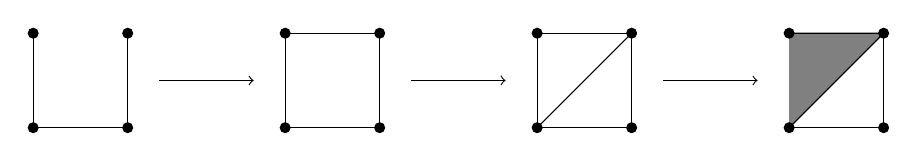
\begin{tikzpicture}[scale=0.4]

  \coordinate (v1) at (0,0);
  \coordinate (v2) at (0,3);
  \coordinate (v3) at (3,0);
  \coordinate (v4) at (3,3);
  \draw (v1) -- (v2);
  \draw (v3) -- (v4);
  \draw (v1) -- (v3);

  \coordinate (w1) at (8+0,0);
  \coordinate (w2) at (8+0,3);
  \coordinate (w3) at (8+3,0);
  \coordinate (w4) at (8+3,3);
  \draw (w1) -- (w2);
  \draw (w3) -- (w4);
  \draw (w1) -- (w3);
  \draw (w2) -- (w4);
  \draw[->] (4,1.5) -- (7,1.5);

  \coordinate (u1) at (16+0,0);
  \coordinate (u2) at (16+0,3);
  \coordinate (u3) at (16+3,0);
  \coordinate (u4) at (16+3,3);
  \draw (u1) -- (u2);
  \draw (u3) -- (u4);
  \draw (u1) -- (u3);
  \draw (u2) -- (u4);
  \draw (u1) -- (u4);
  \draw[->] (12,1.5) -- (15,1.5);

  \coordinate (uu1) at (24+0,0);
  \coordinate (uu2) at (24+0,3);
  \coordinate (uu3) at (24+3,0);
  \coordinate (uu4) at (24+3,3);
  \draw (uu1) -- (uu2);
  \draw (uu3) -- (uu4);
  \draw (uu1) -- (uu3);
  \draw (uu2) -- (uu4);
  \draw (uu1) -- (uu4);
  \filldraw[fill=gray] (uu1) -- (uu4) -- (uu2);
  \draw[->] (20,1.5) -- (23,1.5);

  \foreach \vertex in {v1,v2,v3,v4,w1,w2,w3,w4,
  u1,u2,u3,u4,
  uu1,uu2,uu3,uu4}
    \fill (\vertex) circle (5pt);
\end{tikzpicture}
\caption{Nous continuons à relier et à remplir lorsque le seuil similarité augmente. \textbullet On compte le nombre d'apparitions de trous comme une mesure de la richesse des structures dans une dissertation.}
\label{filtration}
\end{figure}
\end{frame}

\begin{frame}{Analyse sur un ensemble de données réelles}
source de données (plus précisément, l'ensemble d'essais 2, qui est discursif) :
\fontsize{7pt}{8pt}\selectfont
\url{https://www.kaggle.com/datasets/thevirusx3/automated-essay-scoring-dataset/code?select=training_set_rel3.tsv}
\begin{figure}[H]
  \includegraphics[width=5cm]{gradesah1s.png}
  \includegraphics[width=5cm]{gradesah1w.png}
  \caption{La moyenne des trous de chaque phrase/mot augmente avec le niveau scolaire (de 1 à 6, histogramme du haut vers le bas).}
  \label{fig:ads}
\end{figure}
% \vspace{-0.5cm}
% \begin{figure}[H]
% \begin{minipage}[c]{0.67\textwidth}
% \scalebox{0.45}{
  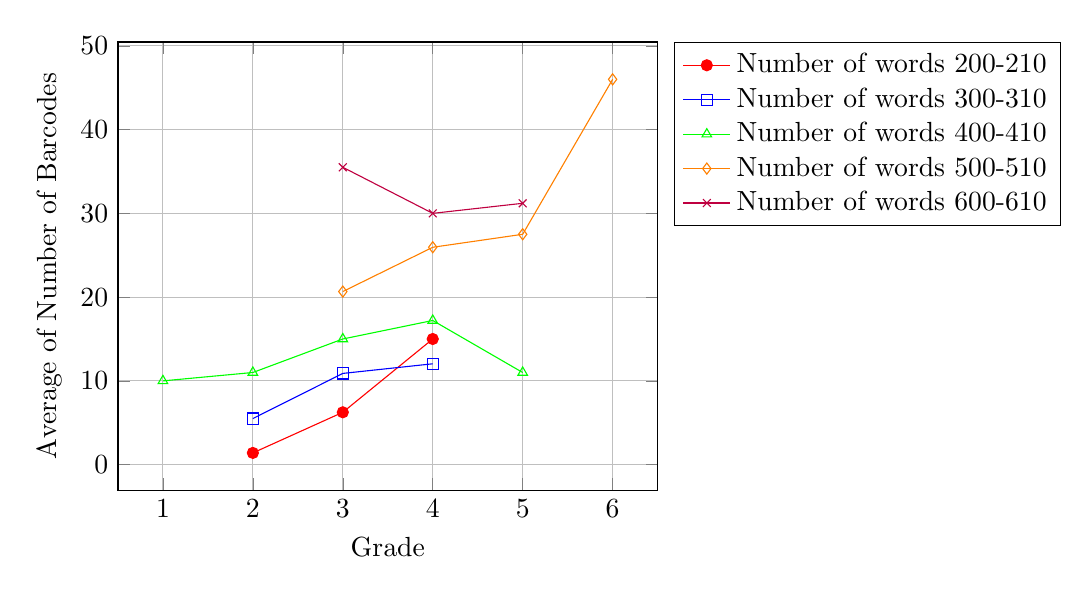
\begin{tikzpicture}
    \begin{axis}[
      xlabel={Grade},
      ylabel={Average of Number of Barcodes},
      legend pos=outer north east,
      grid=both,
    ]
    
    % Number of words 200-210
    \addplot[color=red,mark=*] coordinates {
      (2, 1.4)
      (3, 6.25)
      (4, 15.0)
    };
    
    % Number of words 300-310
    \addplot[color=blue,mark=square] coordinates {
      (2, 5.5)
      (3, 10.89)
      (4, 12.04)
    };
    
    % Number of words 400-410
    \addplot[color=green,mark=triangle] coordinates {
      (1, 10.0)
      (2, 11.0)
      (3, 15.0)
      (4, 17.21)
      (5, 11.0)
    };
    
    % Number of words 500-510
    \addplot[color=orange,mark=diamond] coordinates {
      (3, 20.66)
      (4, 25.95)
      (5, 27.5)
      (6, 46.0)
    };
    
    % Number of words 600-610
    \addplot[color=purple,mark=x] coordinates {
      (3, 35.5)
      (4, 30.0)
      (5, 31.2)
    };
    
    \legend{
      Number of words 200-210,
      Number of words 300-310,
      Number of words 400-410,
      Number of words 500-510,
      Number of words 600-610
    }
    
    \end{axis}
    \end{tikzpicture}
}
% \end{minipage}\hfill
% \begin{minipage}[c]{0.3\textwidth}
% \caption{Notes et moyennes des nombres de trous dans des plages de nombres de mots fixes}
% \end{minipage}\hfill
% \end{figure}

\end{frame}

\section{Outro}
\begin{frame}
\linespread{1}
\setbeamertemplate{itemize/enumerate body begin}{\vspace{0.5pt}}
\frametitle{Analyse - Conclusions}

\begin{columns}[t]
\begin{column}{0.55\textwidth} % Updated width for the first column
\begin{block}{Chargement des données}
\begin{itemize}
\item Gérer un grand jeu de données
\item Décisions sur le prétraitement
\end{itemize}
\end{block}

\begin{block}{Techniques d'apprentissage}
\begin{itemize}
\item Choix de la représentation des données 
\item Choix de la distance
\item Choix du modèle d'apprentissage
\item Importance de la gestion du déséquilibre des classes
\end{itemize}
\end{block}
\end{column}

\begin{column}{0.4\textwidth} % Updated width for the second column
\begin{block}{Limitations et améliorations}
\begin{itemize}
\item Gérer les sentiments subjectifs
\item Défis de l'adaptation au domaine
\item Intervention de l'homologie persistante
\item Exploration de modèles de Deep Learning
\end{itemize}
\end{block}
\end{column}
\end{columns}
\end{frame}
\section{Annexe}
\begin{frame}{Annexe}
\fontsize{7pt}{8pt}\selectfont
\begin{figure}[H]
\begin{minipage}{0.49\linewidth}
\includegraphics[width=4cm]{pdessay.png}
\end{minipage}
\begin{minipage}{0.49\linewidth}
\begin{mdframed}
In @DATE1's world, there are many things found offensive.  Everyone has their own opinion on what is offensive and what is not. Many parents are becoming upset because they think their children are viewing things that they should not.  Other people are upset because they think the libraries are offending their culture or way of life.  This is even taken to the extreme where people want censhorship on libraries to avoid this, which is wrong.     Some people are becoming concerned about the materials in libraries...($\sim$450 words)
\end{mdframed}
\end{minipage}
\caption{Le diagramme de persistance d'un essai de niveau 4/6 : Un point bleu $(x, y)$ dans ce diagramme signifie qu'un trou apparaît à $d=x$ et disparaît à $d=y$.
qu'il y a un trou qui apparaît à $d=x$ et disparaît à $d=y$.
Un point rouge signifie qu'il n'y a qu'une seule composante connectée tout le temps,
parce que nous lions toutes les phrases par ordre dans la dissertation.
}
\label{fig:pd}
\end{figure}
\end{frame}

\begin{frame}{Annexe}
\begin{figure}[H]
\begin{minipage}[c]{0.67\textwidth}
\scalebox{0.45}{
  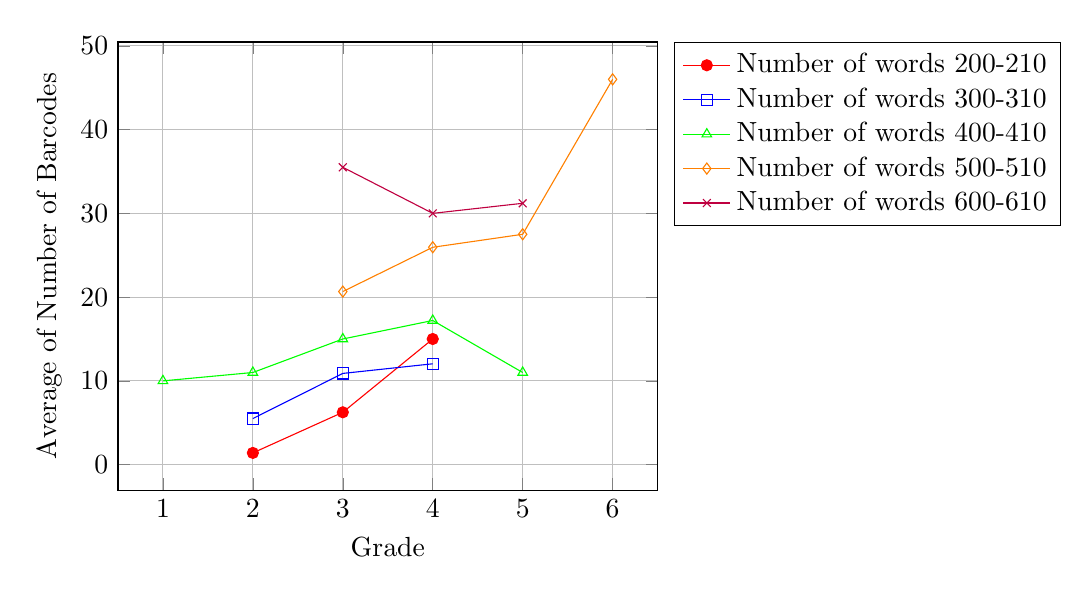
\begin{tikzpicture}
    \begin{axis}[
      xlabel={Grade},
      ylabel={Average of Number of Barcodes},
      legend pos=outer north east,
      grid=both,
    ]
    
    % Number of words 200-210
    \addplot[color=red,mark=*] coordinates {
      (2, 1.4)
      (3, 6.25)
      (4, 15.0)
    };
    
    % Number of words 300-310
    \addplot[color=blue,mark=square] coordinates {
      (2, 5.5)
      (3, 10.89)
      (4, 12.04)
    };
    
    % Number of words 400-410
    \addplot[color=green,mark=triangle] coordinates {
      (1, 10.0)
      (2, 11.0)
      (3, 15.0)
      (4, 17.21)
      (5, 11.0)
    };
    
    % Number of words 500-510
    \addplot[color=orange,mark=diamond] coordinates {
      (3, 20.66)
      (4, 25.95)
      (5, 27.5)
      (6, 46.0)
    };
    
    % Number of words 600-610
    \addplot[color=purple,mark=x] coordinates {
      (3, 35.5)
      (4, 30.0)
      (5, 31.2)
    };
    
    \legend{
      Number of words 200-210,
      Number of words 300-310,
      Number of words 400-410,
      Number of words 500-510,
      Number of words 600-610
    }
    
    \end{axis}
    \end{tikzpicture}
}
\end{minipage}\hfill
\begin{minipage}[c]{0.3\textwidth}
\caption{Notes et moyennes des nombres de trous dans des plages de nombres de mots fixes}
\end{minipage}\hfill
\end{figure}
\end{frame}
\end{document}
